\documentclass[_main.tex]{subfiles}
 
\begin{document}

%%%%%%%%%%%%
\section*{Estimating the quantum of transmission}
\label{main_estimating_Q}
%%%%%%%%%%%%

In this section and the next we explore ways to infer local transmission parameters from measurements of within-host variation.  With modern sequencing technologies it is feasible to measure within-host variation at millions of SNP loci.  For each host, we can calculate the mean of within-host heterozygosity for all nucleotide positions across the genome, $\pi_W$, which is the within-host equivalent of nucleotide diversity.  We will show how this can be used to estimate the quantum of transmission $Q$.

Unlike the coalescent approach used in previous sections, which proceeded backwards in time, we shall now imagine that we are following parasites as they flow along an individual transmission chain, and consider the effects of mutation, genetic drift and superinfection as we proceed forwards in time.  Although this approach requires some approximation and is more cumbersome than the coalescent approach, it provides valuable insights into how the transmission parameters $Q$ and $\chi$ could be estimated by deep sequencing of individual infections.

\paragraph{Within-host heterozygosity in the absence of superinfection.}  

%Consider a transmission chain that never crosses with another transmission chain, i.e. there is no superinfection.  Imagine two hosts that are one generation apart on this transmission chain, i.e. that the first host transmits parasites directly to the second host.  Let $H_W$ be the within-host heterozygosity of the first host and $H'_W$ that of the second at some arbitrary point locus.  As parasites flow from the first to the second host, genetic drift due to the transmission bottleneck will act to reduce heterozygosity, while mutation will act to increase heterozygosity.  Here we will focus on SNP heterozygosity and so the relevant mutation rate is the frequency of single nucleotide substitution $\mu \approx 1.1 \times 10^{-8}$ per generation.  As described in Methods section \ref{supp_whh_chi_0}, the Wright-Fisher model gives us the relationship

Consider a transmission chain that never crosses with another transmission chain, i.e. there is no superinfection.  Imagine two hosts that are $x$ generations apart on this transmission chain.  Let $H_W$ be the within-host heterozygosity of the first host and $H'_W$ that of the second at some arbitrary point locus.  As parasites flow from the first to the second host, genetic drift due to the transmission bottleneck will act to reduce heterozygosity, while mutation will act to increase heterozygosity.  Here we will focus on SNPs so the relevant mutation rate is that of single nucleotide substitution $\mu \approx 1.1 \times 10^{-8}$ per generation.  As described in Methods section \ref{supp_whh_chi_0}, the Wright-Fisher model gives us the relationship


%\begin{equation}
%H'_W \approx H_W \big( 1 - \frac{1}{Q} \big) \big( 1 - 2 \mu \big) + 2 \mu 
%\label{eq:main_hahb}
%\end{equation}

%This is an approximation because we are ignoring factors of $\mu^2$ which are exceedingly small.  Now imagine that the two hosts are $x$ generations apart on the same transmission chain.  If we repeat the above equation over $x$ generations, we obtain

\begin{equation}
H'_W \approx H_W \alpha^x + 2 \mu \sum_{i=0}^{x-1} \alpha^i
\label{eq:main_alpha_decay}
\end{equation}

where

\begin{equation}
\alpha = \big( 1 - \frac{1}{Q} \big) \big( 1 - 2 \mu \big)
\label{eq:main_alpha}
\end{equation}

%The first part of equation \ref{eq:main_alpha_decay} describes geometric decay of the initial heterozygosity due to genetic drift, while the second part describes a new source of heterozygosity that gradually builds up due to the accumulation of mutations, attenuated by drift.  

If we follow this transmission chain over time, it will eventually reach an equilibrium level of within-host heterozygosity as long as it does not cross with another transmission chain.  We can evaluate this equilibrium value by letting $x \rightarrow \infty$ in equation \ref{eq:main_alpha_decay}.  We can get an empirical estimate of this value by using deep sequencing to determine $\pi_W$, the mean within-host heterozygosity at all nucleotide positions in the parasite genome. As shown in Methods section \ref{supp_whh_chi_0}, in the absence of superinfection

\begin{equation}
Q 
\approx \frac{ \pi_W ( 1 - 2 \mu) }{ 2 \mu ( 1 - \pi_W ) }
\approx \frac{ \pi_W }{ 2 \mu }
\label{eq:main_Q_est}
\end{equation}

This is reminiscent of equation \ref{eq:main_Tc_pi} which gave $T_C \approx \pi / 2\mu$.  Here we have a special case of the genomic transmission graph where $T_C = Q$ because we are sampling two alleles that are cotransmitted and because $\chi=0$. 

\paragraph{Inferring $Q$ from measurements of within-host nucleotide diversity $\pi_W$.}  Equation \ref{eq:main_Q_est} provides a way of estimating the quantum of transmission $Q$ by deep sequencing of the parasite genome within individual hosts.  It requires that we sample from hosts who lie on transmission chains that have not experienced superinfection at any time in the recent past.  We would expect this to include a relatively high proportion of hosts in regions with low malaria transmission intensity, e.g. South America, but to be much less common in regions with high transmission intensity such as West Africa.

It is beyond the scope of this paper to carry out a sufficiently detailed analysis of empirical data to make a reliable estimate of the quantum of transmission, but we can make a crude preliminary estimate as proof of concept using genome variation data from a global sample of thousands of malaria-infected individuals produced by the MalariaGEN network \cite{MalariaGEN2021}.  The methods of this preliminary analysis are described in Methods section \ref{supp_Q_pi}.  As shown in figure \ref{fig:main_pi_w_distribution} we find a striking bimodal distribution for $\pi_W$, with the first peak comprising hosts with low $\pi_W$ ($\sim 4 \times 10^{-7}$) and the second peak comprising hosts with high $\pi_W$ ($\sim 5 \times 10^{-5}$).

\begin{figure}[h!]
\centering
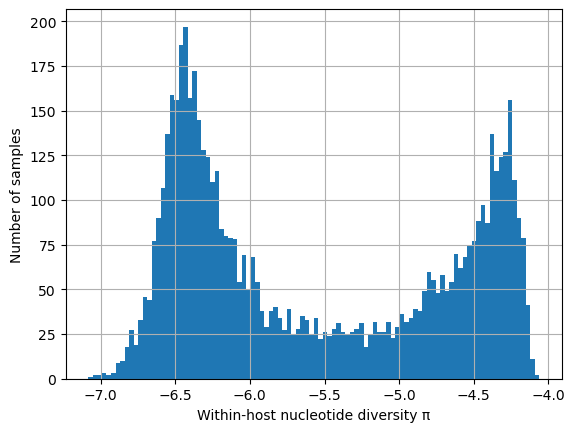
\includegraphics[width=12cm]{230117_wiho_het_0_01.png}
\caption{
\textbf{Distribution of $\pi_W$ in samples from around world.}  Levels of within-host nucleotide diversity obtained from a preliminary analysis of 5970 samples from 30 countries in the MalariaGEN Pf6 dataset \cite{MalariaGEN2021} as described in Methods section \ref{supp_Q_pi}.  This shows that $\pi_W$ has a striking bimodal distribution.
}
\label{fig:main_pi_w_distribution}
\end{figure}

Here we postulate that the high $\pi_W$ peak is caused by hosts with superinfection and cotransmission whereas the low $\pi_W$ peak is caused by hosts that lie on transmission chains that have not experienced superinfection in the recent past.  This interpretation of the data is supported by the observation that the relative heights of the two peaks vary according to the population sampled, with the low $\pi_W$ peak being more prominent in regions of low transmission and the high $\pi_W$ peak more prominent in regions of high transmission, as shown in figure \ref{fig:main_pi_w_regional}. 

\begin{figure}[h!]
\centering
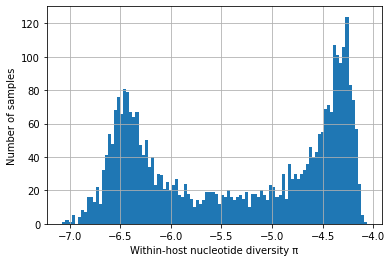
\includegraphics[width=7cm]{230317_wiho_het_Africa.png}
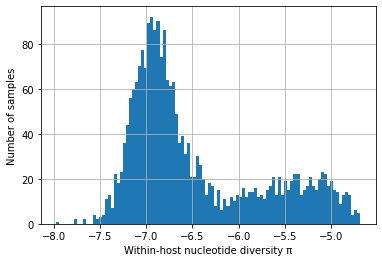
\includegraphics[width=7cm]{230317_wiho_het_SEA.png}
\caption{
\textbf{Distribution of $\pi_W$ in regions with high and low malaria transmission.}  Analysis of 3314 samples from Africa (left panel, high transmission) and 2341 samples from Southeast Asia (right panel, low transmission) in the MalariaGEN  Pf6 dataset \cite{MalariaGEN2021}.  Both regions show a bimodal distribution but the high $\pi_W$ peak is more prominent in West Africa and the low $\pi_W$ peak is more prominent in Southeast Asia.
}
\label{fig:main_pi_w_regional}
\end{figure}

The value of the low $\pi_W$ peak is somewhat higher in Africa ($\sim4 \times 10^{-7}$) than in Southeast Asia ($\sim1.2 \times 10^{-7}$).  If we assume a single nucleotide substitution rate of $\mu \approx 1.1 \times 10^{-8}$ then from equation \ref{eq:main_Q_est} we obtain an estimate of $Q \approx 18$ in Africa and $Q \approx 5$ in Southeast Asia.

An important caveat to this analysis is that genotyping errors could possibly contribute to the low $\pi_W$ peak, which would act to inflate estimates of $Q$.  Ideally we would like to evaluate the rate of within-host genotyping errors by analysing deep sequencing data from duplicate sequencing runs on the same samples, as has been done for SARS-CoV2 \cite{Tonkin-Hill2021}.  In the absence of such data, we have attempted to reduce the number of genotyping errors by analysing only biallelic coding SNPs with good data quality scores.  A potentially important source of error is incorrect alignment of sequence reads to paralogous sequences, giving rise to the phenomenon of hyperheterozygosity as described in reference \cite{Manske2012}.  Therefore we have excluded all SNPs whose within-host heterozygosity is $>2\%$ when averaged across all samples, which greatly reduces the risk of systematic errors of this type, at the cost of potentially deflating our estimates of $\pi_W$.  Other checks to exclude obvious systematic errors in the low $\pi_W$ peak are outlined in Methods section \ref{supp_Q_pi}, but clearly there is a need for replicated deep sequencing data and more detailed analyses in order to obtain a reliable estimate of the quantum of transmission in different epidemiological settings.  

%%%%%%%%%%%%%

%\section{Estimating the crossing rate of transmission chains}

%We shall now consider populations that experience superinfection and explore the question of how to estimate $\chi$.  We define $\chi$ as the crossing rate of transmission chains but it can also be simply described as the proportion of hosts that are superinfected.  From an epidemiological perspective $\chi$ is related to the incidence of infection and the serial interval of transmission, as approximately described in equation x.

%Our approach to this problem stems from a striking empirical observation that was made when it first became possible to measure within-host heterozygosity at a very large number of SNP loci by deep genome sequencing (Figure \ref{fig:hwhs_nature}) \cite{Manske2012}.  For each SNP we can measure both its heterozygosity in the local subpopulation, $H_S$, and its heterozygosity within an individual host, $H_W$.  It was discovered that $H_W$ and $H_S$ show a striking linear correlation when data from a large number of SNPs are analysed within a single infected individual. 

\section*{Understanding the relationship between $H_W$ and $H_S$}
\label{main_section_Hw_Hs}  

When a very large number of SNP loci are analysed by deep genome sequencing of parasite samples from malaria-infected individuals, there is a striking linear correlation between $H_W$ (the heterozygosity of a locus within an individual host) and $H_S$ (the heterozygosity of that locus in the local subpopulation) \cite{Manske2012,Auburn2012}.   This relationship is not apparent if we examine a small number of SNPs in isolation, but it becomes highly statistically significant if we aggregate data on hundreds of thousands of SNPs.

Figure \ref{fig:hwhs_nature} is taken from the study where this phenomenon was first described \cite{Manske2012}.  SNPs are sorted into bins corresponding to different levels of $H_S$ and this is plotted against the mean value of $H_W$ observed for that set of SNPs in an individual host.   The figure shows a series of lines of varying slope, each of which represents the linear relationship between $H_W$ and $H_S$ for an individual host.

\begin{figure}[h!]
\centering
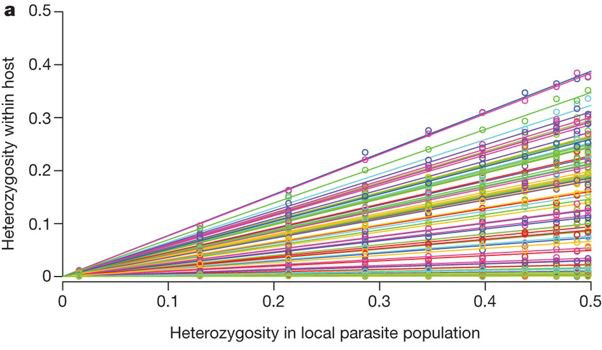
\includegraphics[width=13cm]{180918_hwhs_nature.png}
\caption{\textbf{Empirical relationship between parasite heterozygosity within individual hosts and within the local parasite subpopulation.}  Based on genome sequencing of blood samples from patients with malaria.  Data on 86,000 SNPs were aggregated by placing SNPs into frequency bins based on $H_S$ (heterozygosity in the local parasite population) and then plotting the mean value of $H_W$ (heterozygosity within an individual host).  $H_W$ shows a strong linear correlation with $H_S$ for each sample, but the slope of this line varies greatly between samples. From reference \cite{Manske2012}}
\label{fig:hwhs_nature}
\end{figure}

The slope of this linear relationship varies between infected individuals but there is a pattern to this variation.  At low levels of malaria transmission intensity, $H_W$ tends to be very low and the slope of $H_W$/$H_S$ is close to zero.  At high levels of transmission intensity, there is a much wider range of $H_W$ values and the slope of $H_W$/$H_S$ varies considerably between infected individuals.  If  $\widehat{H}_W$ denotes the mean of $H_W$ in the local subpopulation, we find that the slope of $\widehat{H}_W$/$H_S$ tends to increase with the malaria transmission intensity of the location.

This raises the question of why there is a linear relationship between $\widehat{H}_W$ and $H_S$, and what determines the slope of this relationship.  Here we approach this question by imagining that we are following a transmission chain forward in time as it crosses with other transmission chains.  As we shall see, this leads to insights into how measurements of within-host heterozygosity can be used to estimate $\chi$.

\paragraph{An isolated episode of superinfection.}  Imagine an episode of superinfection in which host C acquires infection from host A and host B.  Let the $Q$ alleles acquired from host A have heterozygosity $H'_A$, and the $Q$ alleles acquired from host B have heterozygosity $H'_B$.  Note that $H'_A$ is not exactly the same as the heterozygosity of host A as it allows for genetic drift and mutation that have occurred in the process of transmission from host A to host C (figure \ref{fig:main_superinfected}).  

\begin{figure}[h!]
\centering
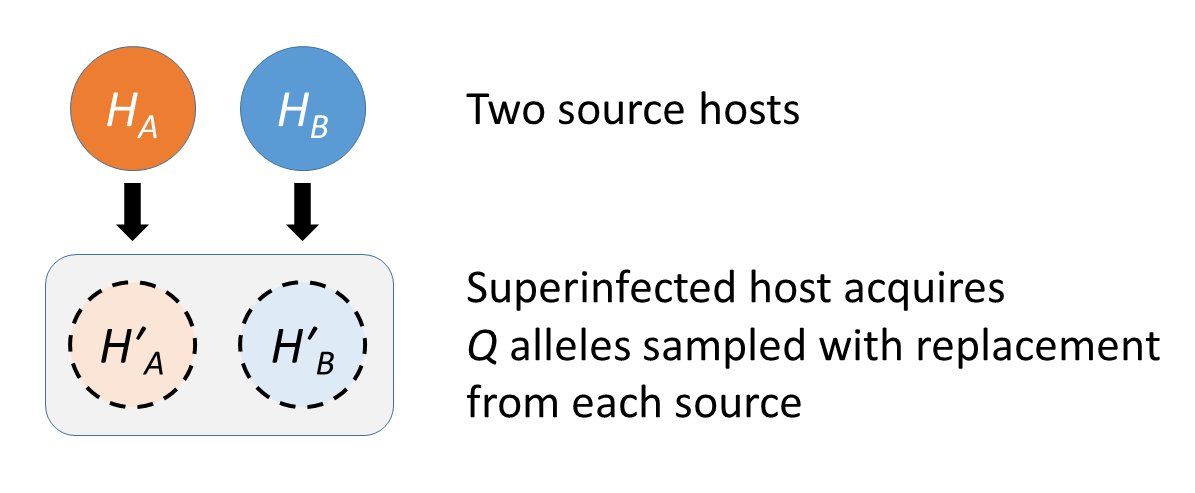
\includegraphics[width=8cm]{210814_superinfection.png}
\caption{\textbf{An episode of superinfection.}  In our idealised transmission graph, a superinfected host acquires $Q$ alleles from each of two source hosts, who have heterozygosity values $H_A$ and $H_B$.  The acquired alleles are sampled with replacement from the source hosts and they are also subject to mutation.  If we know $H_A$ and $H_B$ then we can obtain $H_A'$ and $H_B'$ from equation \ref{eq:main_alpha_decay}.  We obtain the heterozygosity of the superinfected host by sampling without replacement from the pool of $2Q$ acquired alleles.}
\label{fig:main_superinfected}
\end{figure}

To obtain the heterozygosity of host C we must sample two alleles without replacement from the pool of $2Q$ acquired alleles, which themselves were sampled with replacement from host A and host B.  As described in Methods section \ref{supp_episode_superinfection} the heterozygosity of the superinfected host is given by 

\begin{equation}
H_C =
\frac{(Q-1) (H_A' + H_B') }{2(2Q-1)} + \frac{Q H_S}{2Q-1}
\label{eq:crossing_tc_2}
\end{equation}

Thus superinfection typically causes a considerable increase in the within-host heterozygosity of a transmission chain because $H_S$ is generally much greater than $H_A'$ or $H_B'$.  

\paragraph{Recurrent episodes of superinfection along a transmission chain.}  

Now imagine that we are following a transmission chain that crosses with other transmission chains with a probability of $\chi$ per generation.  Let \textbf{X} be a random variable representing the number of generations that separate two crossing events on this transmission chain: 

\begin{equation}
Pr \{ \textbf{X} = i \} = \chi (1- \chi)^{i-1}
\label{eq:main_xprobdist}
\end{equation}

\begin{figure}[h!]
\centering
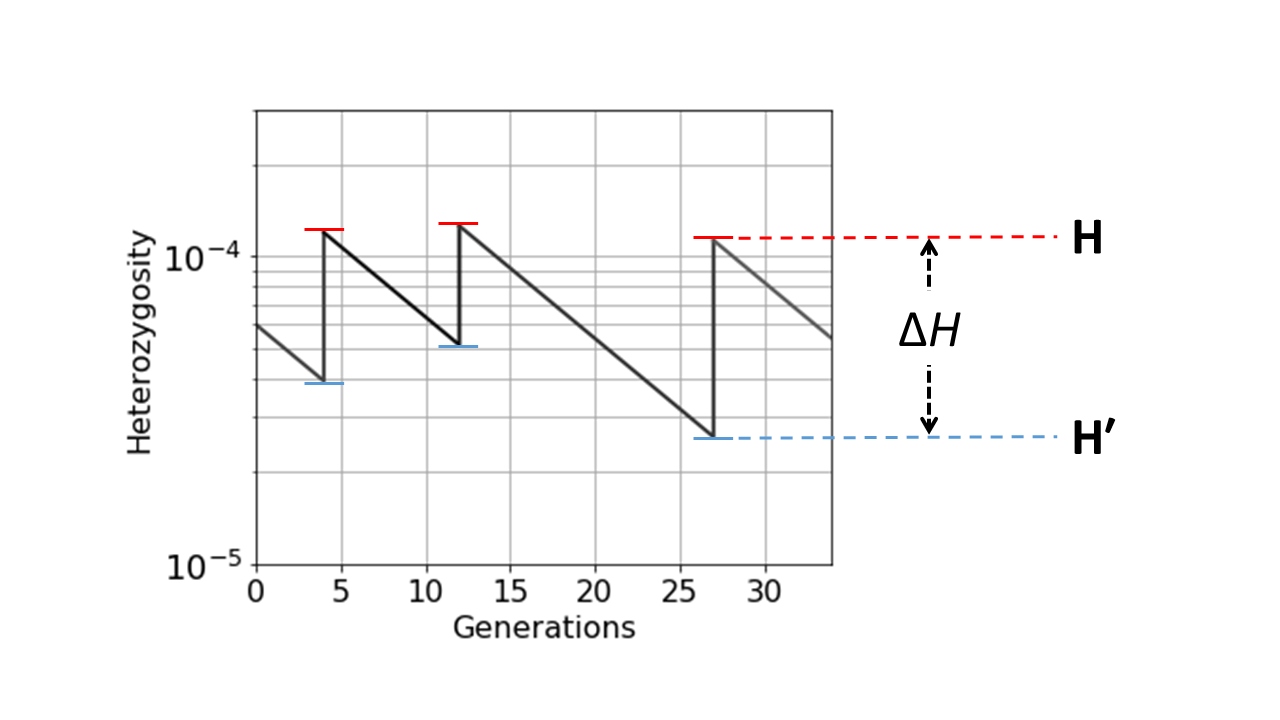
\includegraphics[width=12cm]{181002_random_cross.png}
\caption{
\textbf{A transmission chain that crosses at random intervals with other transmission chains.}  There are large temporal fluctuations in within-host heterozygosity.  Heterozygosity is boosted by each crossing event and then declines gradually due to genetic drift until it is boosted by the next crossing event.  $\mathbf{H}$ and  $\mathbf{H'}$ are random variables representing the peaks and troughs, respectively, of within-host heterozygosity along our transmission chain.   $\Delta H$ is the increase in within-host heterozygosity that occurs as a result of a crossing event.
}
\label{fig:tcrand}
\end{figure}

Each crossing event causes within-host heterozygosity to rise abruptly to a peak, and then genetic drift causes it to decline gradually to a trough before it is boosted by another crossing event, as illustrated in figure \ref{fig:tcrand}.  These peaks and troughs will vary in magnitude according to the number of generations that separate crossing events.  Let $\mathbf{H}$ and  $\mathbf{H'}$ be random variables representing the peaks and troughs, respectively, of within-host heterozygosity along our transmission chain at some arbitrary locus.  We can think of $\mathbf{H'}$ and $\mathbf{H}$ as the states of our transmission chain immediately before and after crossing has occurred in a superinfected host, analogous to $H_A'$ and $H_C$ in equation \ref{eq:crossing_tc_2}.  

Let $\Delta H$ be the increase in within-host heterozygosity that occurs as a result of a crossing event.  If we assume that all transmission chains have the same probability distributions for $\mathbf{H}$ and $\mathbf{H'}$ as our transmission chain, by applying equation \ref{eq:crossing_tc_2} we obtain the expectation of $\Delta H$:

\begin{equation}
\label{eq:main_deltah}
E \{ \mathbf{H} - \mathbf{H'} \} = \frac{Q}{2Q-1} E\{ H_S  - \mathbf{H'} \}
\end{equation}

For the system to be in equilibrium, the expectation of $\Delta H$ must equal the expected decrease in heterozygosity that occurs due to genetic drift in the interval between two crossing events, which we can obtain from equations \ref{eq:main_alpha_decay} and \ref{eq:main_xprobdist}. 

Let $\widehat{H}_W$ be the mean value of within-host heterozygosity across our transmission chain. We can evaluate $\widehat{H}_W$ by utilising equations \ref{eq:main_alpha_decay}, \ref{eq:main_xprobdist} and \ref{eq:main_deltah} and making some approximations, as described in Methods section \ref{derive_hwhs_1}, to obtain this linear relationship between $\widehat{H}_W$ and $H_S$: 

\begin{equation}
\label{eq:main_hwhs}
\widehat{H}_W \approx \kappa H_S + \lambda
\end{equation}

where

\begin{equation*}
\kappa =
\sum_{i=1}^\infty \frac{Q \chi (1-\chi)^{i-1}}{ 2Q - (Q-1) \alpha^i - 1}
\times
\sum_{j=0}^\infty \chi (1 - \chi)^j \alpha^j
\end{equation*}

and

\begin{equation*}
\lambda = 2u \sum_{j=0}^\infty \sum_{k=0}^{j-1}  \chi (1- \chi)^j \alpha^k
\end{equation*}

Since our transmission chain is representative of all transmission chains, $\widehat{H}_W$ is the mean value of within-host heterozygosity for the population as a whole.

This provides a mathematical rationale for the empirically observed relationship between $\widehat{H}_W$ and $H_S$.   The slope of this linear relationship $\kappa$ is determined by $\chi$ and $Q$, and ranges between 0 and 1.  The intercept $\lambda$ is a very small value that represents the accumulation of mutations along a transmission chain in the interval between time of sampling and the most recent crossing event.

\begin{figure}[h!]
\centering
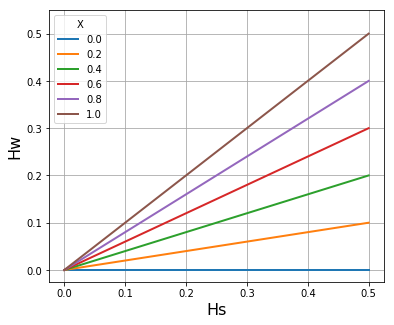
\includegraphics[width=7cm]{221118_hw_vs_hs_Q1.png}
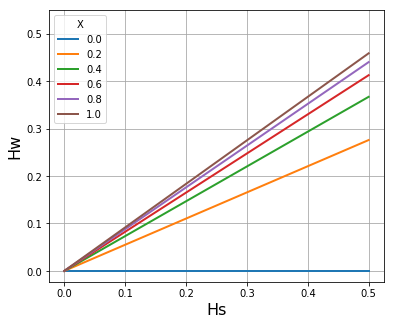
\includegraphics[width=7cm]{221118_hw_vs_hs_Q10.png}
\caption{\textbf{Theoretical relationship between $\widehat{H}_W$ and $H_S$ based on equation \ref{eq:main_hwhs}.}  $\widehat{H}_W$ is the mean of within-host heterozygosity for the local population.  Showing results for $Q = 1$ (left panel) and $Q = 10$ (right panel).  Different lines represent different values of $\chi$ ranging from 0 to 1.  $\widehat{H}_W$ shows a strong linear correlation with $H_S$ and the slope depends on $\chi$ and $Q$.
\href{https://github.com/d-kwiat/gtg/blob/main/hw_vs_hs.ipynb}{View code}
}
\label{fig:hw_vs_hs_model}
\end{figure}

Figure \ref{fig:hw_vs_hs_model} illustrates the linear relationship between $\widehat{H}_W$ and $H_S$ based on equation \ref{eq:main_hwhs}, showing how the slope of the line depends on the combination of $\chi$ and $Q$, being zero if there is no superinfection, i.e. if $\chi = 0$. 

%%%%%%%%%%%%%%%%%%%%%%%%%%%%%

\paragraph{Using $F_{WS}$ to estimate the rate of superinfection $\chi$.}

We can measure the slope of $\widehat{H}_W$ versus $H_S$ by deep genome sequencing of parasites in a sample of infected hosts drawn from the local population, as illustrated in figure \ref{fig:hwhs_nature}.  Equation \ref{eq:main_hwhs} provides a way to use these empirical measurements to estimate $\chi$, particularly if we are able to estimate $Q$ independently using equation \ref{eq:main_Q_est}.

We previously discussed the use of Wright's fixation indices to describe hierarchical population structure and we can extend this concept to within host-diversity if we let $F_{WS} = 1 - \widehat{H}_W / H_S$.  $F_{WS}$ is analogous to an inbreeding coefficient that measures deviation from random mating.  For parasite populations, the primary cause of non-random mating is compartmentalisation of the population into discrete transmission chains that do not cross, although there might be other contributory factors such as gametocyte mating bias.  In the special case of $\chi = 1$ and $Q = 1$, the genomic transmission graph has properties similar to a randomly mating diploid population, with $\widehat{H}_W / H_S = 1$ and $F_{WS} = 0$, i.e. this is analogous to Hardy-Weinberg equilibrium.

It is arbitrary whether we use $\widehat{H}_W / H_S$ or $F_{WS} = 1 - \widehat{H}_W / H_S$ to summarise measurements of within-host variation by deep sequencing, but $F_{WS}$ is now commonly used in the literature and we shall follow that practice here.  In general $F_{WS}$ is inversely related to transmission intensity \cite{Auburn2012,Manske2012,MalariaGEN2021} and is broadly correlated with complexity of infection, i.e. the number of distinct parasite haplotypes detected within a sample \cite{Auburn2012}.  However there is the possibility that $F_{WS}$ could be confounded by population structure as discussed in Methods section \ref{supp_fws_pop_structure}.

A key question is whether equation \ref{eq:main_hwhs} gives the same result as Markov chain simulation in describing the relationship of $F_{WS}$ to $\chi$ and $Q$.  Figure \ref{fig:main_fws_compare_methods} compares the two methods.  This confirms that they give essentially the same results when the effective number of hosts is large, but the results deviate when the effective number of hosts is small.  This is to be expected as the simplifying assumptions used to derive equation \ref{eq:main_hwhs} depend on the number of transmission chains being relatively large.

%%%%%%%%%%%%%%%%%%%%%%%

\begin{figure}[h!]
\centering
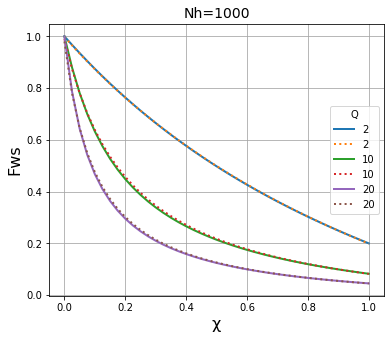
\includegraphics[width=7cm]{221115_fws_compare_1000.png}
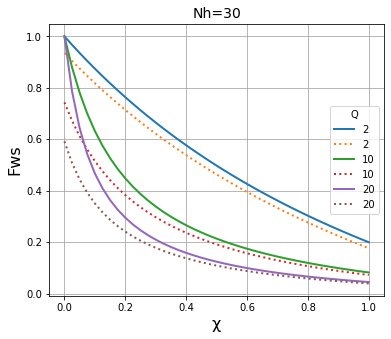
\includegraphics[width=7cm]{221115_fws_compare_30.png}
\caption{\textbf{The inbreeding coefficient $F_{WS}$ is inversely related to $\chi$.}  Colours represent different values of $Q$.  Solid lines show the results obtained from equation \ref{eq:main_hwhs} and dotted lines show the results obtained by Markov chain simulation of coalescence times.  When $N_h=1000$ (left panel) the two methods give very similar results.  When $N_h = 30$ (right panel) equation \ref{eq:main_hwhs} tends to overestimate $F_{WS}$ at low values of $\chi$ as compared with the results obtained by Markov chain simulation.  Methods section \ref{supp_compare_methods} shows results for other values of $N_h$.
\href{https://github.com/d-kwiat/gtg/blob/main/fws_compare_methods.ipynb}{View code}
}
\label{fig:main_fws_compare_methods}
\end{figure}

%%%%%%%%%%%%%%%%%%%%%%%

\begin{figure}[h!]
\centering
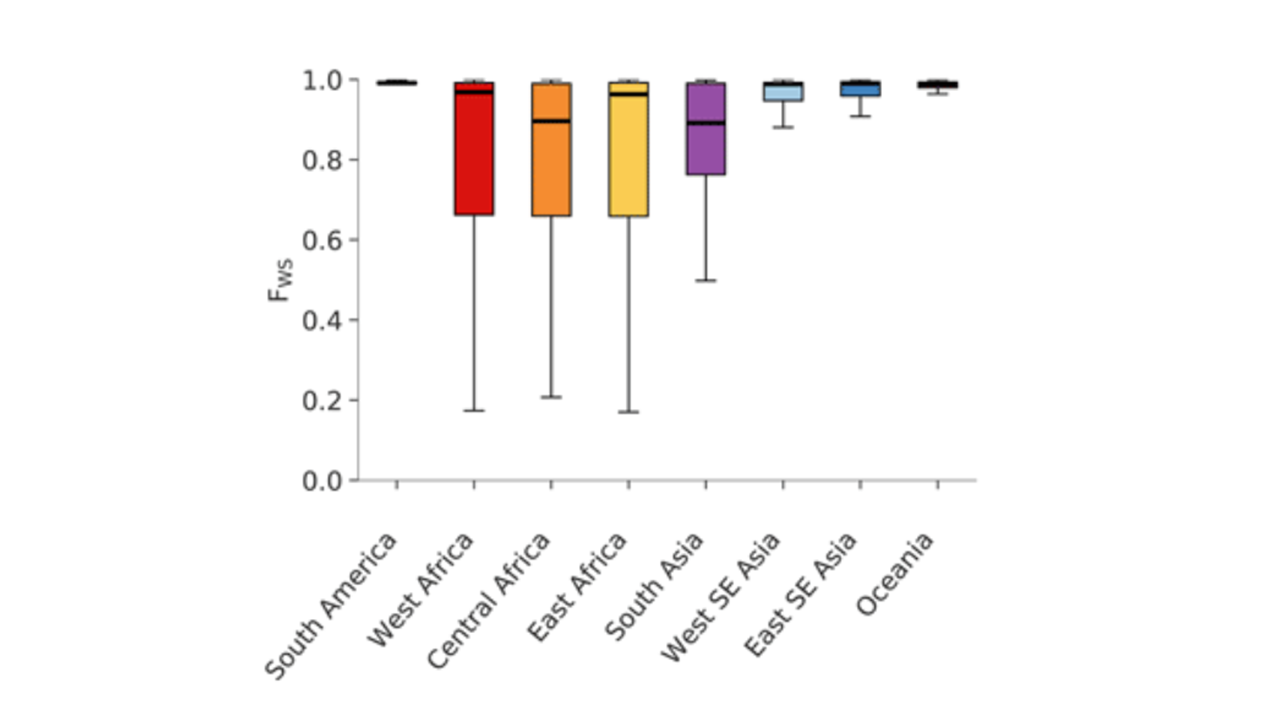
\includegraphics[width=13cm]{221228_Fws_Pf6_final.png}
\caption{\textbf{Estimates of $F_{WS}$ from deep genome sequencing of \textit{P. falciparum} samples}.  This figure is taken from the MalariaGEN Pf6 dataset (reference \cite{MalariaGEN2021} fig. 2) which analysed 5,970 samples from locations around the world.  Thick lines represent median values, boxes show the interquartile range, and whiskers represent the bulk of the distribution, discounting outliers.  
}
\label{fig:Fws_Pf6_figure}
\end{figure}

Thus empirical measurements of $F_{WS}$ allow us to estimate $\chi$, particularly if we are also able to estimate $Q$ using equation \ref{eq:main_Q_est}.  Figure \ref{fig:Fws_Pf6_figure} shows typical measurements of $F_{WS}$ in different malaria-endemic regions of the world.  In South America, where levels of malaria transmission are relatively low, $F_{WS} > 0.98$ in the majority of samples, and from figure \ref{fig:main_fws_compare_methods} this implies that $\chi < 0.02$.  

In contrast, in Central Africa $F_{WS}$ is much more variable between samples, ranging from 0.2 to 1 with a median value of $\sim 0.9$, i.e. the distribution is very assymetrical.  If both $Q$ and $N_h$ are relatively large this implies that $\chi < 0.1$, whereas if $Q$ and $N_h$ are small this implies that $\chi \approx 0.1$. 

This is a somewhat remarkable result.  It implies that, even in regions of high malaria transmission, where at least half of all samples show evidence of multiclonal infections, only a small minority of samples ($\leq 0.1$) are actually superinfected.   This means that the majority of multiclonal infections are due to cotransmission rather than superinfection.  It is consistent with recent findings from single cell genome sequencing studies in Malawi that cotransmission of related parasites is much more common than superinfection, and that complex infections can undergo serial passage through multiple hosts without loss of diversity \cite{Nkhoma2020}.

\end{document}